\documentclass[english]{beamer}

\usepackage{fontspec}
\setmainfont{Calibri}
\setsansfont{Calibri}

\setcounter{secnumdepth}{3}
\setcounter{tocdepth}{3}
\setlength{\parskip}{\smallskipamount}
\setlength{\parindent}{0pt}
\usepackage{graphicx}

\usepackage{xcolor}

\def\redcolor{\color{red}}
\def\blackcolor{\color{black}}
\def\bluecolor{\color{blue}}

\usepackage{minted}
%\newminted{verilog}{breaklines}
\newminted{verilog}{breaklines,fontsize=\small}
\newminted{text}{breaklines,fontsize=\small}


\title{Pengenalan FPGA}
\author{Fadjar Fathurrahman}
\date{}

\begin{document}

\frame{\titlepage}


\begin{frame}
\frametitle{FPGA (Field Programmable Gate Arrays)}

{\centering
%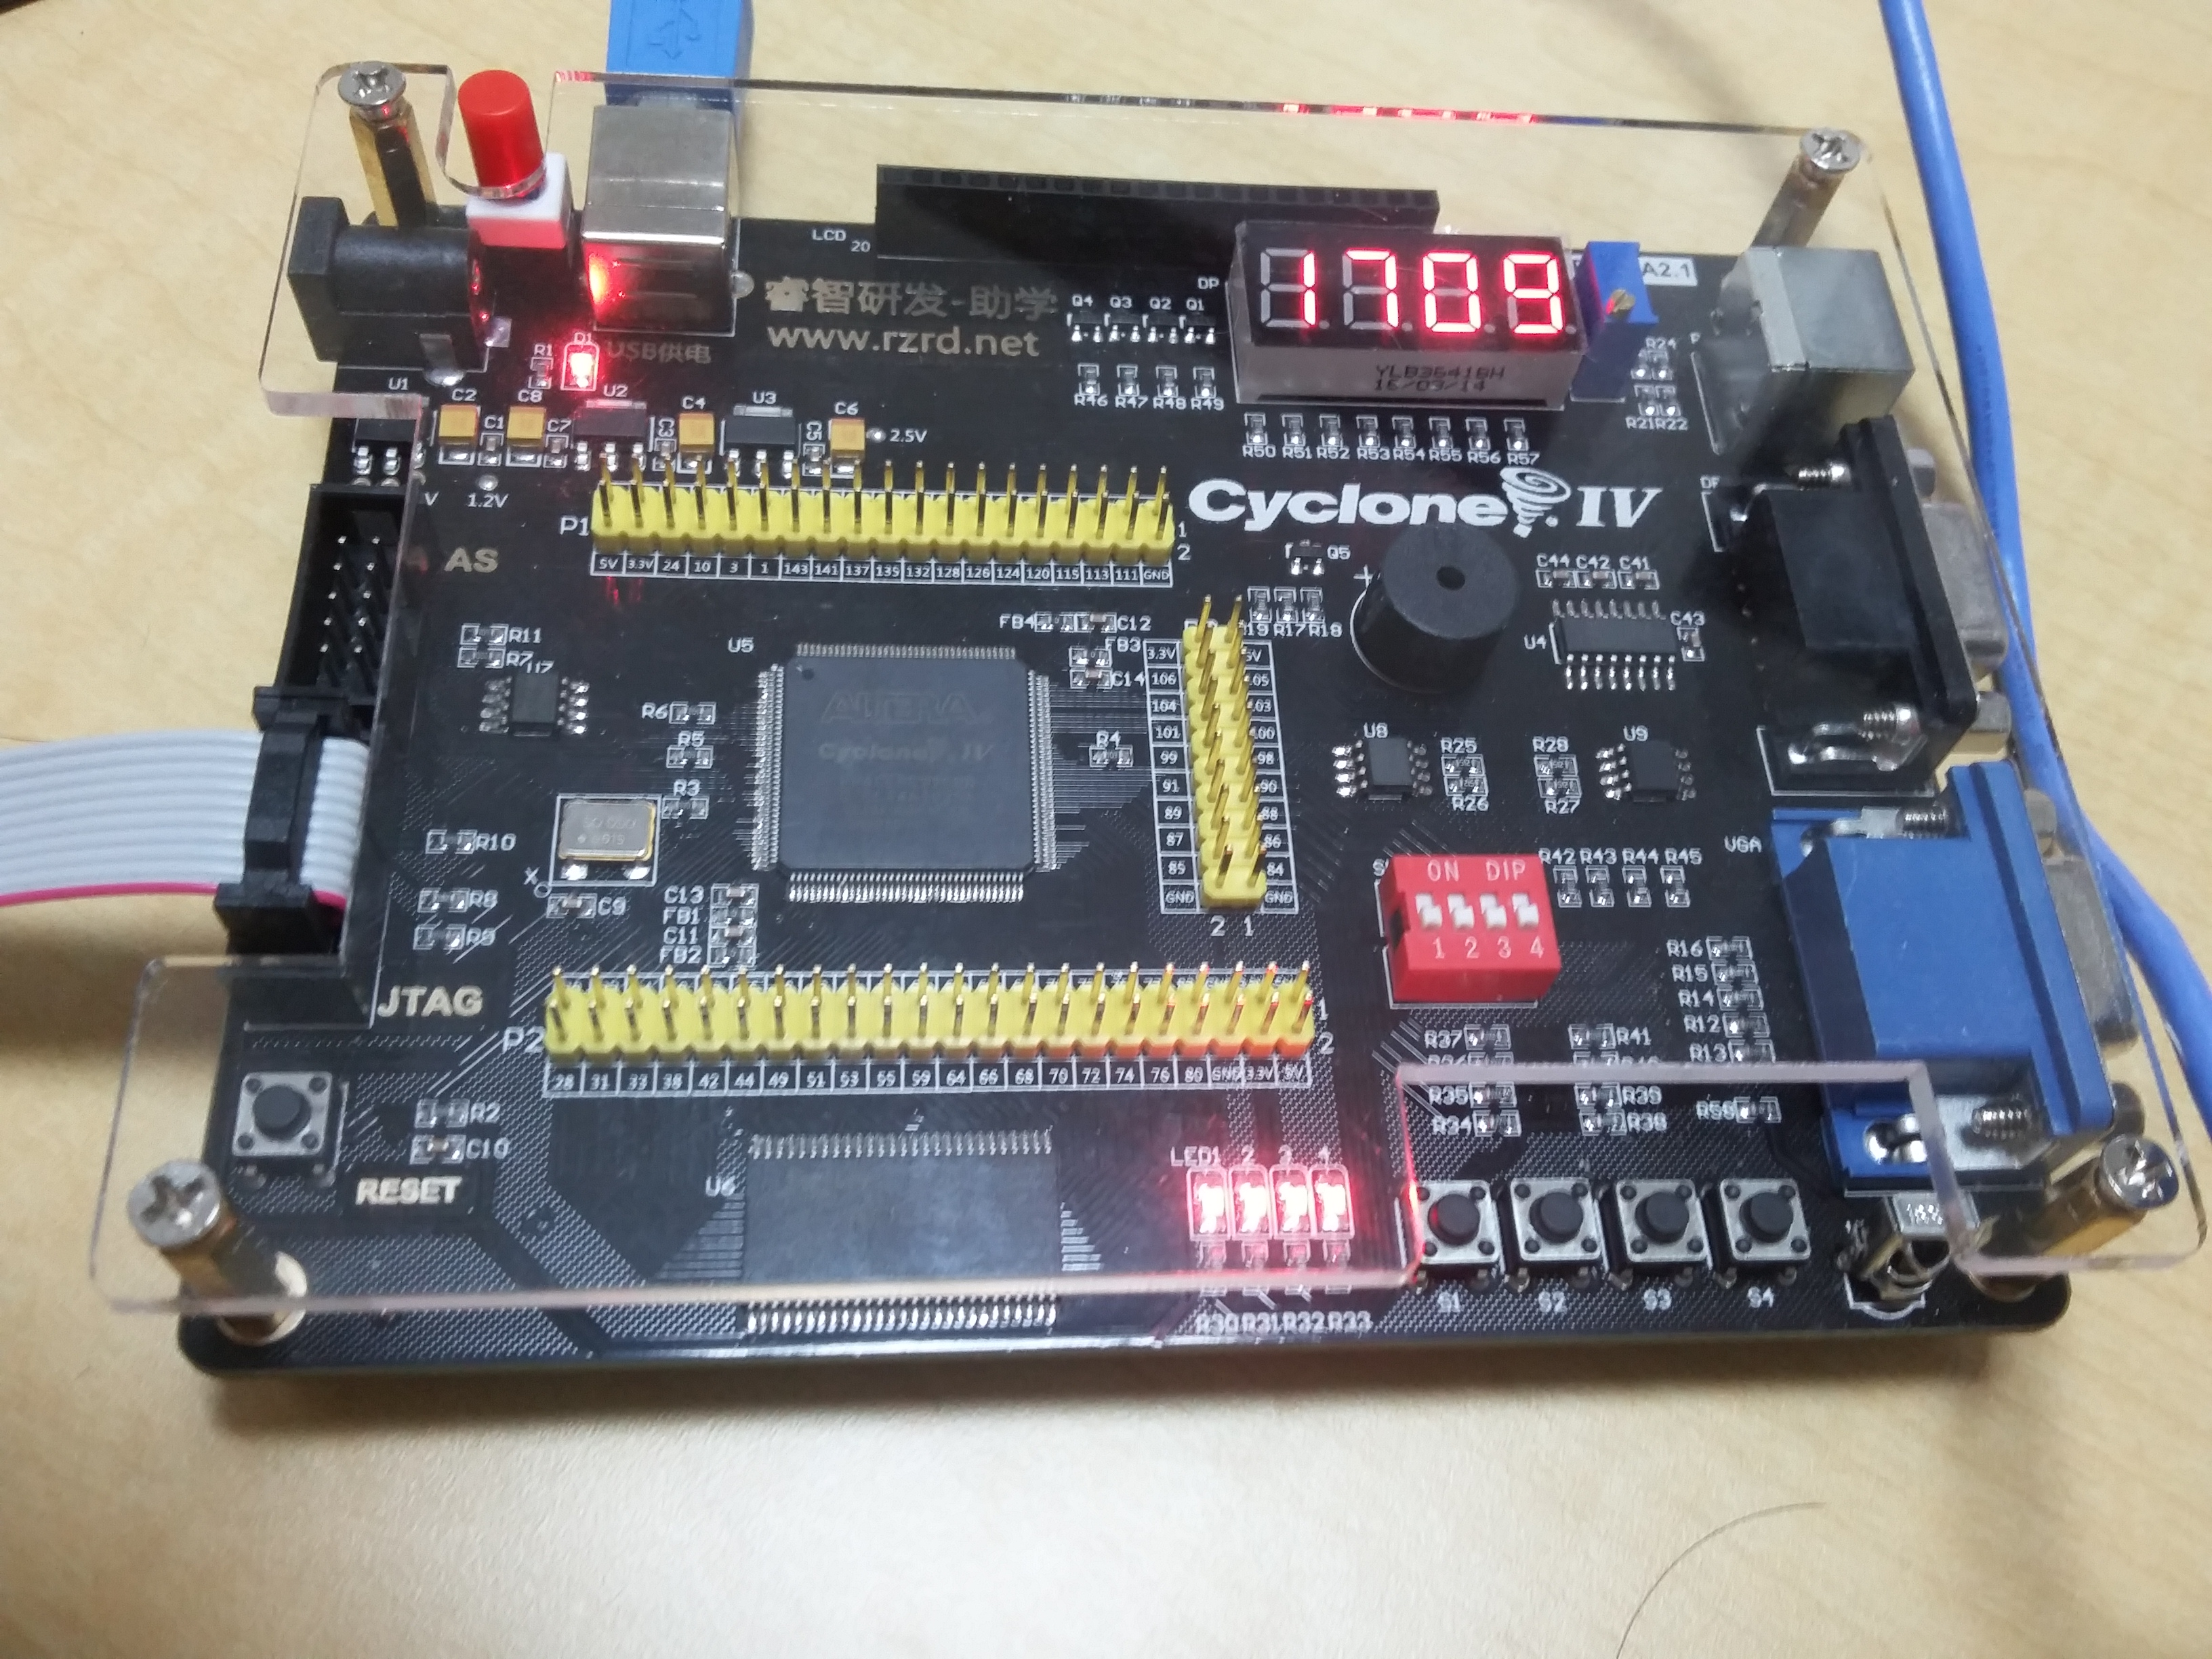
\includegraphics[width=0.75\textwidth]{../images/foto_FPGA_v1.jpg}
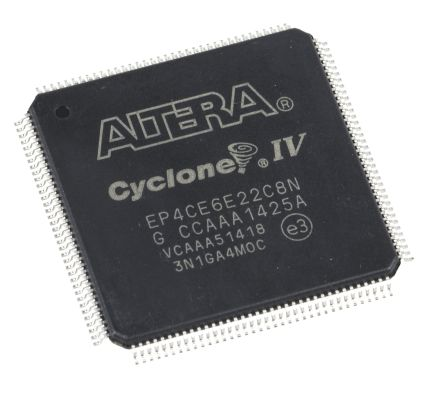
\includegraphics[width=0.5\textwidth]{../images/altera_cyclone_iv.jpg}
\par}

\end{frame}


\begin{frame}
\frametitle{FPGA}

FPGA merupakan rangkaian terintegrasi yang dapat dikonfigurasi oleh pengguna
setelah proses manufaktur dari pabrik.

Pada FPGA, kita diberikan kumpulan gerbang logika yang dapat dikonfigurasi
untuk sesuai dengan kebutuhan.

(Apa perbedaannya dengan mikrokontroler?)

Beberapa aplikasi FPGA:
\begin{itemize}
\item \textit{prototyping} sistem digital
\item pengontrol
\item pemrosesan sinyal, gambar, dll
\item high performance computing
\end{itemize}


\end{frame}




\begin{frame}
\frametitle{Pemrograman FPGA}

Beberapa cara untuk memprogram FPGA

\begin{itemize}
\item skematik
\item bahasa deskripsi hardware (HDL: hardware description language): Verilog,
VHDL, \textit{etc}.
\end{itemize}

\end{frame}


\begin{frame}
\frametitle{Altera: Quartus}

\end{frame}


\begin{frame}[fragile]
\frametitle{Verilog code}

Test
\begin{verilogcode}
module bcd2sseg(
  input wire s1,
  input wire s0,
  output [7:0] sseg );
  
  sseg[0] = s1 & s2;

endmodule
\end{verilogcode}



\end{frame}


\end{document}


